
\documentclass[a4paper,11pt]{article}
\usepackage[a4paper, margin=8em]{geometry}

% usa i pacchetti per la scrittura in italiano
\usepackage[french,italian]{babel}
\usepackage[T1]{fontenc}
\usepackage[utf8]{inputenc}
\frenchspacing 

% usa i pacchetti per la formattazione matematica
\usepackage{amsmath, amssymb, amsthm, amsfonts}

% usa altri pacchetti
\usepackage{gensymb}
\usepackage{hyperref}
\usepackage{standalone}

% imposta il titolo
\title{Appunti Fondamenti di Automatica}
\author{Luca Seggiani}
\date{2025}

% disegni
\usepackage{pgfplots}
\pgfplotsset{width=10cm,compat=1.9}

% imposta lo stile
% usa helvetica
\usepackage[scaled]{helvet}
% usa palatino
\usepackage{palatino}
% usa un font monospazio guardabile
\usepackage{lmodern}

% tikz in sans
\tikzset{every picture/.style={/utils/exec={\sffamily}}}

\renewcommand{\rmdefault}{ppl}
\renewcommand{\sfdefault}{phv}
\renewcommand{\ttdefault}{lmtt}

% circuiti
\usepackage{circuitikz}
\usetikzlibrary{babel}

% disponi il titolo
\makeatletter
\renewcommand{\maketitle} {
	\begin{center} 
		\begin{minipage}[t]{.8\textwidth}
			\textsf{\huge\bfseries \@title} 
		\end{minipage}%
		\begin{minipage}[t]{.2\textwidth}
			\raggedleft \vspace{-1.65em}
			\textsf{\small \@author} \vfill
			\textsf{\small \@date}
		\end{minipage}
		\par
	\end{center}

	\thispagestyle{empty}
	\pagestyle{fancy}
}
\makeatother

% disponi teoremi
\usepackage{tcolorbox}
\newtcolorbox[auto counter, number within=section]{theorem}[2][]{%
	colback=blue!10, 
	colframe=blue!40!black, 
	sharp corners=northwest,
	fonttitle=\sffamily\bfseries, 
	title=Teorema~\thetcbcounter: #2, 
	#1
}

% disponi definizioni
\newtcolorbox[auto counter, number within=section]{definition}[2][]{%
	colback=red!10,
	colframe=red!40!black,
	sharp corners=northwest,
	fonttitle=\sffamily\bfseries,
	title=Definizione~\thetcbcounter: #2,
	#1
}

% disponi problemi
\newtcolorbox[auto counter, number within=section]{problem}[2][]{%
	colback=green!10,
	colframe=green!40!black,
	sharp corners=northwest,
	fonttitle=\sffamily\bfseries,
	title=Problema~\thetcbcounter: #2,
	#1
}

% disponi codice
\usepackage{listings}
\usepackage[table]{xcolor}

\lstdefinestyle{codestyle}{
		backgroundcolor=\color{black!5}, 
		commentstyle=\color{codegreen},
		keywordstyle=\bfseries\color{magenta},
		numberstyle=\sffamily\tiny\color{black!60},
		stringstyle=\color{green!50!black},
		basicstyle=\ttfamily\footnotesize,
		breakatwhitespace=false,         
		breaklines=true,                 
		captionpos=b,                    
		keepspaces=true,                 
		numbers=left,                    
		numbersep=5pt,                  
		showspaces=false,                
		showstringspaces=false,
		showtabs=false,                  
		tabsize=2
}

\lstdefinestyle{shellstyle}{
		backgroundcolor=\color{black!5}, 
		basicstyle=\ttfamily\footnotesize\color{black}, 
		commentstyle=\color{black}, 
		keywordstyle=\color{black},
		numberstyle=\color{black!5},
		stringstyle=\color{black}, 
		showspaces=false,
		showstringspaces=false, 
		showtabs=false, 
		tabsize=2, 
		numbers=none, 
		breaklines=true
}

\lstdefinelanguage{javascript}{
	keywords={typeof, new, true, false, catch, function, return, null, catch, switch, var, if, in, while, do, else, case, break},
	keywordstyle=\color{blue}\bfseries,
	ndkeywords={class, export, boolean, throw, implements, import, this},
	ndkeywordstyle=\color{darkgray}\bfseries,
	identifierstyle=\color{black},
	sensitive=false,
	comment=[l]{//},
	morecomment=[s]{/*}{*/},
	commentstyle=\color{purple}\ttfamily,
	stringstyle=\color{red}\ttfamily,
	morestring=[b]',
	morestring=[b]"
}

% disponi sezioni
\usepackage{titlesec}

\titleformat{\section}
	{\sffamily\Large\bfseries} 
	{\thesection}{1em}{} 
\titleformat{\subsection}
	{\sffamily\large\bfseries}   
	{\thesubsection}{1em}{} 
\titleformat{\subsubsection}
	{\sffamily\normalsize\bfseries} 
	{\thesubsubsection}{1em}{}

% disponi alberi
\usepackage{forest}

\forestset{
	rectstyle/.style={
		for tree={rectangle,draw,font=\large\sffamily}
	},
	roundstyle/.style={
		for tree={circle,draw,font=\large}
	}
}

% disponi algoritmi
\usepackage{algorithm}
\usepackage{algorithmic}
\makeatletter
\renewcommand{\ALG@name}{Algoritmo}
\makeatother

% disponi numeri di pagina
\usepackage{fancyhdr}
\fancyhf{} 
\fancyfoot[L]{\sffamily{\thepage}}

\makeatletter
\fancyhead[L]{\raisebox{1ex}[0pt][0pt]{\sffamily{\@title \ \@date}}} 
\fancyhead[R]{\raisebox{1ex}[0pt][0pt]{\sffamily{\@author}}}
\makeatother

\begin{document}

% sezione (data)
\section{Lezione del 04-03-25}

% stili pagina
\thispagestyle{empty}
\pagestyle{fancy}

% testo
Avevamo ricavato la formula per la \textbf{risposta libera} di un sistema.
Introduciamo quindi la parte di soluzione legata alla \textbf{risposta forzata} del sistema, cioè quella legata al termine $Bu$ nell'equazione differenziale:
$$
x' = Ax + Bu
$$
da cui:
$$
x(t) = x_l + x_v = e^{At} x_0 + \int_0^t e^{A(t - \tau)} Bu(\tau) \, d\tau
$$
dove la risposta libera è data dal primo termine:
$$
x_l = e^{At} x_0 
$$
e la risposta forzata è data dall'\textit{integrale di convoluzione}:
$$
x_v = \int_0^t e^{A(t - \tau)} Bu(\tau) \, d\tau
$$

\subsection{Caratterizzazione delle variabili di stato}
Vediamo nel dettaglio come si ricavano le variabili di stato $x'$.
Riprendiamo la forma generale del sistema a variabili di stato.
In sostanza avremo una forma differenziale implicita per l'ingresso e l'uscita: 
$$
F \left( y(t), ..., y^{(n)}(t), u(t), ..., u^{(p)}(t), t \right) = 0
$$
da cui possiamo ricavare la derivata di grado massimo dell'uscita: 
$$
y^{(n)}(t) = \hat{F} \left( y(t), ..., y^{n-1}(t), u(t), ..., u^p(t), t \right)
$$

\par\smallskip

Facciamo alcune considerazioni sulla forma di queste equazioni.
Possiamo prendere la forma generale della $F$, che assumiamo rappresentare  un vincolo differenziale che lega in forma implicita ingresso e uscita:
$$
F(t) = \sum_{i = 0}^{n} \alpha_i y^{(i)} (t) + \sum_{j = 1}^{p} \beta_i u^{(j)} (t), \quad F(t) = 0
$$
l'equazione della $y^{(n)} (t)$ sarà allora:
$$
y^{(n)} (t) = \frac{1}{\alpha_n} \left( \sum_{i = 0}^{n - 1} - \alpha_i y^{(i)} (t) + \sum_{j = 0}^p - \beta_i u^{(j)} (t) \right)
$$

Possiamo porre:
\[
	\begin{cases}		
		\alpha_i ' = \frac{\alpha_i}{\alpha_n} \\ 
		\beta_i ' = - \frac{\beta_i}{\alpha_n}
	\end{cases}
\]
in modo da riscrivere la derivata di grado massimo nella forma più compatta:
$$
y^{(n)} (t) = \sum_{i = 0}^{n - 1} - \alpha_i ' y^{(i)} (t) + \sum_{j = 0}^p  \beta_i ' u^{(j)} (t) 
$$
Per questo motivo, da qui in poi assumeremo $\alpha_i \leftarrow \alpha_i '$ e $\beta_i \leftarrow \beta_i '$.

\par\smallskip

Quello che volevamo fare era quindi ricondurci alla forma in variabili di stato:
\[
	\begin{cases}
		x' = Ax + Bu \\ 
		y = Cx + Du
	\end{cases}
\]
a cui siamo abituati.

Il passaggio era quindi quello di riportarci a:
$$
x'(t) = \begin{pmatrix}
x'_1(t) \\
... \\
x'_n(t)
\end{pmatrix}
= \begin{pmatrix}
f_1(t) \\
... \\
f_n(t)
\end{pmatrix}
$$
e date $x$ e $f$ lineari dire:
$$
x'(t) = Ax + Bu
$$

Patiamo dal vettore di stato:
$$
x = \begin{pmatrix}
x_1 \\
... \\
x_n
\end{pmatrix}
= \begin{pmatrix}
y \\
... \\
y^{(n - 1)}
\end{pmatrix}
$$

A questo punto la derivata di $x$ sarà, assunto $p = 0$ (quindi non ci sono derivate dell'ingresso): 
$$
x' = \begin{pmatrix}
x'_1 \\
... \\
x'_n
\end{pmatrix} = \begin{pmatrix}
x_2 \\
... \\
x_n \\ 
y^{(n)}(t)
\end{pmatrix}
= \begin{pmatrix}
x_2 \\
... \\
x_n \\
\hat{F} \left( (y, ..., y^{(n - 1)}), u, t \right)
\end{pmatrix}
= \overline{f}(x, u, t)
$$
che nel caso lineare si riconduce a:
\[
	\begin{cases}	
x' = \left(\begin{array}{@{}c | cccc@{}}
	0 & 1 & 0 & ... & 0 \\
	0 & 0 & 1 & ... & 0 \\
	... & ... & ... & ... & ... \\
	0 & 0 & 0 & ... & 1 \\
	\hline
	-\alpha_0 & ... & ... & ... & -\alpha_{n - 1}
\end{array}\right)
x + \begin{pmatrix}
0 \\
... \\
0 \\
\beta_0
\end{pmatrix} u, \quad p = 0 \\ 
y = \begin{pmatrix}
	1 & 0 & ... & 0
\end{pmatrix} x + \begin{pmatrix}
0
\end{pmatrix} u
	\end{cases}
\]

La matrice $A$ viene detta \textit{compagna orizzontale inferiore}, e i suoi autovalori sono coincidenti alle radici del polinomio $\alpha_0 + \alpha_1 \lambda + ... + \alpha_{n - 1} \lambda^{n - 1} + \lambda^n$ (questo risulta chiaro dallo sviluppo di Laplace sull'ultima riga).

\par\smallskip

Notiamo che questo processo non è dissimile a quello adottato ad esempio nello studio dei sistemi meccanici, dove le derivate successive della posizione facevano da variabili di stato (solitamente posizione e velocità), una di queste variabili faceva da valore di uscita (solitamente la posizione), e la derivata della variabile di stato di ordine più alto (solitamente l'accelerazione) era l'unica derivata della variabile di stato che introduceva nuove informazioni nel sistema.

\subsubsection{Esempio numerico: sistema massa-molla-smorzatore}
Un sistema di questo tipo è stato già studiato nell'esempio 2.3.4, dove avevamo la differenziale che descriveva un carrellino in un sistema molla-smorzatore soggetto ad una forza $F$:
$$
F(t) = M \frac{dv}{dt} + Bv + Kx
$$
che manipolavamo per ottenere la modellizzazione:
$$
A = \begin{pmatrix}
	0 & 1 \\ 
	-\frac{K}{M} & -\frac{B}{M}
\end{pmatrix}, \quad 
B = \begin{pmatrix}
	0 \\ \frac{1}{M}
\end{pmatrix}
$$
$$
C = \begin{pmatrix}
	1 & 0
\end{pmatrix}, \quad 
D = \begin{pmatrix}
0
\end{pmatrix}
$$

Osserviamo che questa è la stessa modellizzazione che avremmo ottenuto applicando il metodo descritto sopra.

Possiamo definire un programma Python che sfrutta la libreria \href{http://scipy.org}{SciPy} per effettuare la simulazione in dominio tempo del sistema:
\lstset{style=codestyle, language=python}
\lstinputlisting{../py/state_variable_form/solve_svf.py}

Proviamo allora a simulare il sistema con valori $m = 5 \, \mathrm{kg}$, $k = 3 \, \frac{\mathrm{N}}{\mathrm{m}}$ e $b = 3 \, \frac{\mathrm{N}}{\mathrm{m}^2}$, da cui le matrici:
$$
A = \begin{pmatrix}
	0 & 1 \\ 
	-0.6 & -0.4
\end{pmatrix}, \quad 
B = \begin{pmatrix}
	0 \\ 0.2
\end{pmatrix}
$$
$$
C = \begin{pmatrix}
	1 & 0
\end{pmatrix}, \quad 
D = \begin{pmatrix}
0
\end{pmatrix}
$$

Vediamo ad esempio lo scalino unitario applicato all'istante $5 \, \mathrm{s}$:
\begin{center}
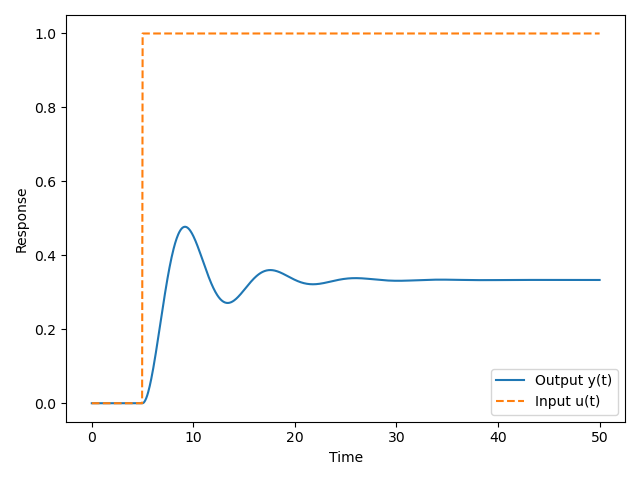
\includegraphics[scale=0.8]{../figures/mass-spring-damper-response.png}
\end{center}

Notiamo che allo stato di regime si avrà $x'' = x' = 0$ (assunta $x$ la posizione del carrello).
In questo caso la differenziale si ridurrà a:
$$
Kx = F \implies x = \frac{F}{K}
$$
che con i dati forniti dà $\sim 0.33 \, \mathrm{m}$, che come notiamo dalla figura è esattamente il punto attorno a cui il sistema si stabilizza.

\subsection{Dipendenza dalle derivate della variabile di ingresso}
Abbiamo posto finora $p = 0$, quindi nessuna derivata della variabili di ingresso.
Vediamo il caso in cui includiamo tali derivate.

\subsubsection{Caso $\mathbf{p < n}$}
Vediamo innanzitutto il caso in cui il termine di grado massimo delle variabili di stato dipende dalle derivate della variabile di ingresso, cioè $0 < p < n$.
Avevamo l'equazione differenziale:
$$
y^{(n)} (t) = \sum_{i=0}^{n-1} - \alpha_i y^{(i)}(t) + \sum_{j=0}^p \beta_j u^{(j)}(t)
$$

In questo caso la situazione si complica, e ci conviene sfruttare il \textbf{principio di sovrapposizione}.
Definiamo l'equazione ausiliaria in $z$:
$$
z^{(n)}(t) = \sum_{i = 0}^{n - 1} -\alpha_i z^{(i)}(t) + u(t)
$$
che rappresenta la risposta del sistema al solo ingresso $u(t)$ (senza derivate superiori).
Vediamo che questa è la forma che siamo stati abituati a risolvere finora.

Sarà quindi vero che la \textit{funzione forzante} (l'ingresso non scalato e non derivato) $u(t)$ porterà alla \textit{soluzione particolare} $z(t)$, cosa che indichiamo come:
$$
\mathcal{H}[u(t)] = z(t) 
$$

Considerando la linearità del sistema, siamo liberi di moltiplicare e derivare per ricavare le risposte alle funzioni derivate successive dell'ingresso scalate per i $\beta_i$ che avevamo nell'equazione originale:
\[
	\begin{cases}
		\mathcal{H}[\beta_0 u(t)] = \beta_0 z(t) \\ 
		\mathcal{H}[\beta_1 u'(t)] = \beta_1 z'(t) \\ 
		... \\
		\mathcal{H}[\beta_p u^{(p)}(t)] = \beta_p z^{(p)}(t)
	\end{cases}
\]

Per ottenere la risposta complessiva del sistema, allora, basterà applicare nuovamente la linearità e prendere la combinazione lineare delle risposte ai singoli ingressi:
$$
y(t) = \sum_{j = 0}^{p} \beta_j z^{(j)}(t)
$$
da cui il sistema finale:
\[
	\begin{cases}	
x' = \left(\begin{array}{@{}c | cccc@{}}
	0 & 1 & 0 & ... & 0 \\
	0 & 0 & 1 & ... & 0 \\
	... & ... & ... & ... & ... \\
	0 & 0 & 0 & ... & 1 \\
	\hline
	-\alpha_0 & ... & ... & ... & -\alpha_{n - 1}
\end{array}\right)
x + \begin{pmatrix}
0 \\
... \\
0 \\
1
\end{pmatrix} u \\ 
y = \begin{pmatrix}
	\beta_0 & ... & \beta_p & 0 & ... & 0
\end{pmatrix} x + \begin{pmatrix}
0
\end{pmatrix} u
	\end{cases}
\]

\subsubsection{Esempio: differenziale con derivata prima dell'ingresso}
Applichiamo il metodo appena visto per l'equazione differenziale:
$$
y'' + y = 2u + u'
$$
Notiamo il termine di derivata prima dell'ingresso $u$.
Riportandoci nella forma $y^{(n)}(t) = \hat{F}$ avremo:
$$
y'' = - y + 2u + u'
$$
con la formula al primo grado:
$$
y'' = -y + u
$$
da cui il sistema:
\[
	\begin{cases}
		\begin{pmatrix}
			x_1' \\ x_2'
		\end{pmatrix}
		=
		\begin{pmatrix}
			0 & 1 \\ 
			-1 & 0
		\end{pmatrix}
		\begin{pmatrix}
			x_1 \\ x_2
		\end{pmatrix}
		+
		\begin{pmatrix}
		0 \\ 1
		\end{pmatrix}
		u \\ 

		y = 
		\begin{pmatrix}
			2 & 1
		\end{pmatrix}
		\begin{pmatrix}
			x_1 \\ x_2
		\end{pmatrix}
		+
		\begin{pmatrix}
			0
		\end{pmatrix}
		u
	\end{cases}
\]
che sappiamo poter calcolare usando la formula di Lagrange.
In seguito vedremo un esempio di calcolo esplicito (esempio 5.0.3) per una certa configurazione di ingressi e stato iniziale.

\subsubsection{Caso $\mathbf{p = n}$}
Vediamo quindi il caso $p = n$. 
Qui avremo l'equazione differenziale:
$$
y^{(n)} (t) = \sum_{i=0}^{n-1} - \alpha_i y^{(i)}(t) + \sum_{j=0}^n \beta_j u^{(j)}(t)
$$
e la dimensione di $C$ non sarà abbastanza da contenere tutti i termini $\beta_i$.
Potremo allora definire la stessa equazione ausiliaria di prima:
$$
z^{(n)}(t) = \sum_{i = 0}^{n - 1} -\alpha_i z^{(i)}(t) + u(t)
$$
e sostituire, dopo aver preventivamente separato l'$n$-esimo termine:
$$
y(t) = \sum_{i = 1}^n \beta_{i - 1} x_i + \beta^n z^{(n)} = \sum_{i = 1}^n \beta_{i - 1} x_i + \beta_n \sum_{i = 1}^{n} -\alpha_{i - 1} z^{(i)}(t) + \beta_n u(t)
$$
da cui:
\[
	\begin{cases}	
x' = \left(\begin{array}{@{}c | cccc@{}}
	0 & 1 & 0 & ... & 0 \\
	0 & 0 & 1 & ... & 0 \\
	... & ... & ... & ... & ... \\
	0 & 0 & 0 & ... & 1 \\
	\hline
	-\alpha_0 & ... & ... & ... & -\alpha_{n - 1}
\end{array}\right)
x + \begin{pmatrix}
0 \\
... \\
0 \\
1
\end{pmatrix} u \\ 
y = \begin{pmatrix}
	\beta_0 - \beta_n \alpha_0 & ... & \beta_{n - 1} - \beta_n \alpha_{n - 1}	
\end{pmatrix} x + \begin{pmatrix}
\beta_n
\end{pmatrix} u
	\end{cases}
\]

\subsection{Rappresentazioni equivalenti}
Vediamo che la scelta di variabili di stato non è unica.
Potremmo infatti avere:
\[
	\begin{cases}
		x' = Ax + Bu \\
		y = Cx + Du
	\end{cases}
\]
e definire una matrice $T \in \mathbb{R}^{n \times n}$ invertibile detta \textbf{matrice del cambio di base} tale che:
$$
\hat{x} = Tx \implies 
\begin{cases}
	\hat{x}' = \hat{A}\hat{x} + \hat{B}u \\
	\hat{y} = \hat{C}\hat{x} + \hat{D}u
\end{cases}
$$

Ricaviamo le matrici $\hat{A}$, $\hat{B}$, $\hat{C}$ e $\hat{D}$ come:
$$
\hat{A} = T A T^{-1}, \quad \hat{B} = TB, \quad \hat{C} = CT^{-1}, \quad \hat{D} = D
$$
visto che:
\[
	\begin{cases}
		T x = T A T^{-1} T x + T B u \\ 
		y = C T^{-1} T x + D u
	\end{cases}
\]
per cancellazione di $T^{-1} T$.

Meccanicamente, questo non significa altro che possiamo prendere diversi sistemi riferimento per velocità e posizione e conservare comunque l'informazione del sistema.

\subsection{Autovalori e modi}
Avevamo dalla formula di Lagrange che per la risposta libera, cioè la soluzione di $x_l' = Ax_l$, è:
$$
	x_l(t) = e^{A(t / t_0)}x_l(t_0)
$$
posta una condizione iniziale a $t = t_0$.

Esistono 2 casi:
\begin{itemize}
	\item A \textit{diagonalizzabile};
	\item A \textit{non diagonalizzabile}.
\end{itemize}

Vediamo questi casi nel dettaglio.

\subsubsection{A diagonalizzabile}
Potremo ricavare una matrice di cambio di base $T$ tale che $A$ risulti diagonale, cioè:
$$
A = T^{-1} A_D T, \quad A_D = \begin{pmatrix}
	\lambda_1 & 0 & 0 \\
	0 & ... & 0 \\
	0 & 0 & \lambda_n
\end{pmatrix}
$$
con $A_D$ detta \textbf{matrice degli autovettori}, dove le entrate delle diagonali sono gli autovalori $A$.

In questo caso possiamo riscrivere lo stato sfruttando la serie di Taylor:
$$
\hat{x_l}(t) = e^{A_Dt} \hat{x_l}_0 = \sum_{k = 0}^\infty \frac{(A_D t)^k}{k!}\hat{x_l}_0
$$
dove la forma diagonale di $A_D$ ci permette di calcolare velocemente $A_D^k$:
$$
A_D^k = \begin{pmatrix}
	\lambda_1^k & 0 & 0 \\
	0 & ... & 0 \\
	0 & 0 & \lambda_n^k
\end{pmatrix}
$$
da cui:
$$
\hat{x_l}(t) = \mathrm{diag} \left\{ \sum_{k = 0}^\infty \frac{(\lambda_1 t)^k}{k!}, ... , \sum_{k = 0}^\infty \frac{(\lambda_n t)^k}{k!} \right\} \hat{x_l}_0
= \mathrm{diag} \left\{ e^{\lambda_1 t}, ..., e^{\lambda_n t} \right\} \hat{x_l}_0
$$
riportandoci nelle coordinate originali avremo:
$$
x_l(t) = T^{-1} \hat{x}(t) = T^{-1} \mathrm{diag} \left\{ e^{\lambda_1 t}, ..., e^{\lambda_n t} \right\} \hat{x_l}_0 = T^{-1} \mathrm{diag} \left\{ e^{\lambda_1 t}, ..., e^{\lambda_n t} \right\} T x_l(t_0)
$$

Chiamiamo gli $e^{\lambda_i}$ \textbf{modi} del sistema.
La funzioni di uscita in assenza di derivate dell'ingresso sarà quindi data da una combinazione lineare dei \textit{modi propri} del sistema:
$$
y_l(t) = C T^{-1} \mathrm{diag} \left\{ e^{\lambda_1 t}, ..., e^{\lambda_n t} \right\} T x_l(t_0)
$$

Notiamo che, come avevamo già osservato, sarà vero che $\lambda = \sigma + i \omega \in \mathbb{C}$, e quindi:
$$
e^{\lambda t} = e^{\sigma t} \cos(\omega t + \phi)
$$
dalla formula di Eulero.

\par\smallskip

Notiamo che i modi di un sistema rappresentano vari "comportamenti" naturali del sistema, che possono essere esponenziali, oscillatori o una loro combinazione sulla base del autovalore corrispondente $\lambda_i$.

Il comportamento complessivo del sistema sarà quindi dato da una qualche combinazione lineare di questi modi.

\subsubsection{A non diagonalizzabile}
Nel caso $A$ non sia diagonalizzabile si può comunque trasformare nella cosiddetta forma di \textbf{Jordan}.
Questa avrà una struttura quasi diagonale, con entrate di valore 1 immediatamente sopra la diagonale. 

In questo caso i modi assumeranno la forma:
$$
t^{\eta - 1}e^{\lambda_i} t
$$
dove $t^{\eta - 1}$ sarà un'intero compreso tra $1$ e la massima dimensione dei \textit{miniblocchi di Jordan} associati all'autovalore.

\end{document}
